\input{preamble.tex}

\usetikzlibrary {datavisualization}

\newcommand{\tableaucroise}[4]{
\begin{tabular}{|c|c|c|c|}
	\cline{2-4}
	\multicolumn{1}{c|}{} & #1 \\ \hline
	#2 \\ \hline
	#3  \\ \hline
	#4  \\ \hline
\end{tabular}
}

\begin{document}

\reversemarginpar

\pagestyle{fancy}
\fancyhead[L]{Terminale STMG}
\fancyhead[C]{\textbf{DS n°7a : probabilités conditionnelles}}
\fancyhead[R]{\today}

\null\vspace{-30pt}
Nom / Prénom : \\

Consignes particulières : 
\begin{itemize}[label=$\bullet$]
	\item 
	La calculatrice est {autorisée}.
	\item 
	Les exercices \ref{exe:1a} et \ref{exe:2a} peuvent être faits partiellement sur la feuille.
	\item 
	Toute trace de recherche est prise en compte.
\end{itemize}

\hrule

\exe{5}{
On considère deux évènements $A$ et $B$ et on donne :
\begin{multicols}{2}
\begin{enumerate}[label=(\roman*)]
\item $P_{\widebar{B}}(A) = 0,8$
\item $P_B(A) = 0,4$
\item $P(\widebar{B}) = 0,3$
\end{enumerate}
\end{multicols}
\begin{enumerate}
\item
Compléter l'arbre ci-dessous :
\begin{center}
\begin{tikzpicture}[scale=1]
\node {}[grow=right, level distance=4cm, sibling distance=2cm]
	child {node {\small $\widebar{B}$}[level distance=4cm, sibling distance=1cm]
		child {node{\small $\widebar{A}$}			
		}
		child {node{\small $A$}
		}
	}
	child {node {\small $B$}[level distance=4cm, sibling distance=1cm]
		child {node{\small $\widebar{A}$}
		}
		child {node{\small $A$}
		}
	}
;
\end{tikzpicture}
\end{center}
\begin{multicols}{2}
\item Calculer $P(A \cap B)$.
\item Calculer $P(\overline{A} \cap \overline{B})$.
\item  Calculer $P(A)$.
\item Calculer $P_A(B)$.
\end{multicols}
\end{enumerate}
}{exe:1a}{
\begin{enumerate}
\item
\begin{center}
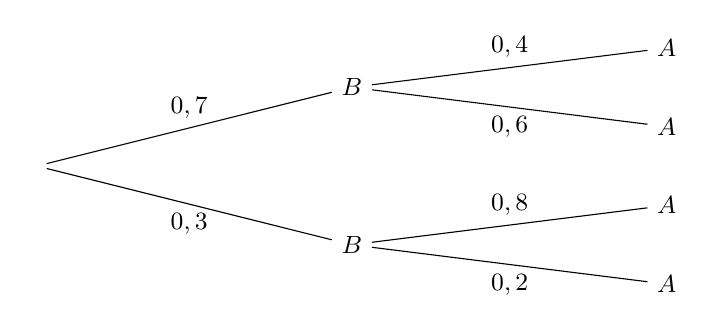
\begin{tikzpicture}[scale=1]
\node {}[grow=right, level distance=4cm, sibling distance=2cm]
	child {node {\small $\widebar{B}$}[level distance=4cm, sibling distance=1cm]
		child {node{\small $\widebar{A}$}
			edge from parent node[below] {\small $0,2$}				
		}
		child {node{\small $A$}
			edge from parent node[above] {\small $0,8$}	
		}
		edge from parent node[below] {\small $0,3$}	
	}
	child {node {\small $B$}[level distance=4cm, sibling distance=1cm]
		child {node{\small $\widebar{A}$}
			edge from parent node[below] {\small $0,6$}	
		}
		child {node{\small $A$}
			edge from parent node[above] {\small $0,4$}
		}
		edge from parent node[above] {\small $0,7$}	
	}
;
\end{tikzpicture}
\end{center}
\begin{multicols}{2}
\item $P(A \cap B) = 0,7 \times 0,4 = 0,28$.
\item $P(\overline{A} \cap \overline{B}) = 0,3 \times 0,2 = 0,06$.
\item $P(A) = 0,7 \times 0,4 + 0,3 \times 0,8 = 0,52$.
\item $P_A(B) = \dfrac{P(B)}{P(A)} P_B(A) = \dfrac{0,7}{0,52} \times 0,4 \approx 0,54$.
\end{multicols}
\end{enumerate}
}

\exe{5}{
Des scientifiques s'intéressent à la population de poissons d'un lac.
Sur les 2~250 individus, 530 sont des ombles, le reste sont des poissons chats.
Parmi les poissons chats, 810 sont des femelles. Il y a en tout 1~300 poissons femelles.
\begin{enumerate}
\item Compléter le tableau croisé d'effectifs ci-dessous :
	\begin{center}
	%\def\arraystretch{1.8}
	\setlength\tabcolsep{20pt}
	\tableaucroise{Femelle & Male & Total}{Omble & & &}{Poisson chat & & &}{Total &&&}
	\end{center}
\item Un scientifique pêche aléatoirement un poisson du lac, estimer (à $10^{-2}$ près) :
\begin{enumerate}
\item la probabilité de pêcher un omble ;
\item la probabilité de pêcher un omble sachant que le poisson est un mâle ;
\item la probabilité de pêcher un poisson chat sachant que le poisson est un mâle.
\end{enumerate}
\item Les évènements \og pêcher un mâle \fg{} et \og pêcher un omble \fg{} sont-ils indépendants ? Justifier.
\end{enumerate}
}{exe:2a}{
\begin{enumerate}
\item
	\begin{center}
	%\def\arraystretch{1.8}
	\setlength\tabcolsep{20pt}
	\tableaucroise{Femelle & Male & Total}{Omble & 490 & 40 & 530}{Poisson chat & 810 & 910 & 1~720}{Total & 1~300 & 950 & 2~250}
	\end{center}
\item
\begin{enumerate}
\item Environ 24 \%.
\item Environ 4 \%.
\item Environ 96 \%.
\end{enumerate}
\item On voit que la probabilité de pêcher un omble et la probabilité de pêcher un omble sachant que c'est un mâle
sont différentes, donc non les évènements sont dépendants.
\end{enumerate}
}

\exe{5}{
On observe un chat. On constate que si la journée est ensoleillée, il chasse (et capture) un lézard 9 fois sur 10. 
Sinon, il n'attrape un lézard que 4 fois sur 10.
On note $p$ la probabilité que la journée soit ensoleillée ainsi que $E$ et $L$ les évènements :
\begin{enumerate}[label=(\roman*)]
\item E : \og la journée est ensoleillée \fg{};
\item L : \og le chat attrape un lézard \fg.
\end{enumerate}
\begin{enumerate} 
\item Construire l'arbre pondéré représentant cette situation.
\item Montrer que $P(L) = 0,5p + 0,4$.
\item On constate que dans 70 \% des cas, le chat attrape un lézard.
\begin{enumerate}
\item Calculer la valeur de $p$. 
\item Sachant qu'il y a 365 jours dans l'année, estimer le nombre de jours ensoleillés. 
\end{enumerate}
\end{enumerate}
}{exe:3a}{
\begin{enumerate} 
\item 

\begin{center}
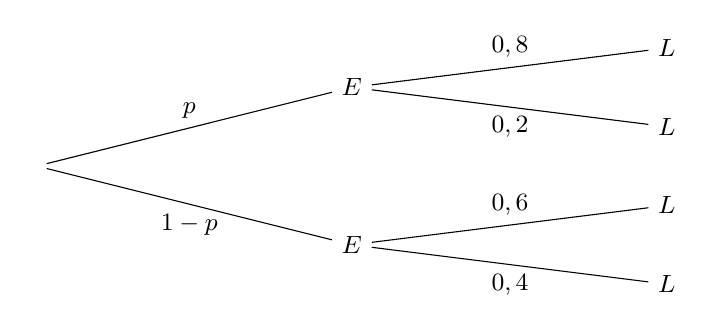
\begin{tikzpicture}[scale=1]
\node {}[grow=right, level distance=4cm, sibling distance=2cm]
	child {node {\small $\widebar{E}$}[level distance=4cm, sibling distance=1cm]
		child {node{\small $\widebar{L}$}
			edge from parent node[below] {\small $0,4$}			
		}
		child {node{\small $L$}
			edge from parent node[above] {\small $0,6$}	
		}
		edge from parent node[below] {\small $1-p$}
	}
	child {node {\small $E$}[level distance=4cm, sibling distance=1cm]
		child {node{\small $\widebar{L}$}
			edge from parent node[below] {\small $0,2$}
		}
		child {node{\small $L$}
			edge from parent node[above] {\small $0,8$}
		}
		edge from parent node[above] {\small $p$}
	}
;
\end{tikzpicture}
\end{center}

\item On a 
\[ P(L) = P(L \cap E) + P(L \cap \overline{E}) = 0,9p + 0,4(1-p) = 0,5p + 0,4 . \]
\item 
\begin{enumerate}
\item Si $P(L) = 0,7$ alors $0,7 = 0,5p + 0,4$ et $p=0,6$.
\item Environ 60 \% de l'année soit 219 jours.
\end{enumerate}
\end{enumerate}
}

\exe{5}{
Des sportifs passent un contrôle anti-dopage à l'issue d'une compétition sportive. On considère les deux évènements suivants :
\begin{enumerate}[label=(\roman*)]
\item
$D$ : \og Le sportif est dopé \fg. 
\item
$T$ : \og Le résultat du test est positif \fg. 
\end{enumerate}
La probabilité qu'un sportif soit testé positif sachant qu'il est dopé est de 95 \%. \\
La probabilité qu'un sportif soit testé positif sachant qu'il n'est pas dopé est de 5 \%.
\begin{enumerate}
\item On donne $P(D \cap T) = 0,019$ en déduire $P(D)$.
\item Représenter la situation par un arbre de probabilité.
\item Calculer la probabilité qu'un sportif soit testé positif.
\item Calculer la probabilité d'un sportif soit dopé sachant qu'il est testé positif.
\item Commenter la qualité du test mis en oeuvre.
\end{enumerate}
}{exe:4a}{

\begin{enumerate}
\item 
On a :
\[ P(D \cap T) = P_D(T) \cdot P(D) =  0,019 \] 
avec $P_D(T) = 0,95$, soit : 
\[ P(D) = \dfrac{0,019}{0,95} = 0,02 . \] 
\item 

\begin{center}
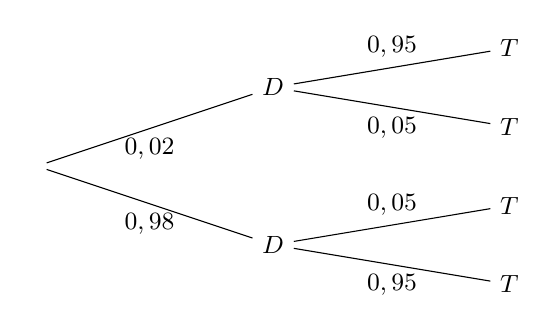
\begin{tikzpicture}[
  grow=right,
  level 1/.style={level distance=3cm, sibling distance=2cm},
  level 2/.style={level distance=3cm, sibling distance=1cm},
]

\node {}
	child {
		node {\small $\widebar{D}$}
		child {
			node {\small $\widebar{T}$}
			edge from parent node[below] {\small $0,95$}
		}
		child {
			node {\small $T$}
			edge from parent node[above] {\small $0,05$}
		}
		edge from parent node[below] {\small $0,98$}
	}
	child {
		node {\small $D$}
		child {
			node {\small $\widebar{T}$}
			edge from parent node[below] {\small $0,05$}
		}
		child {
			node {\small $T$}
			edge from parent node[above] {\small $0,95$}
		}
		edge from parent node[below] {\small $0,02$}
	};
\end{tikzpicture}
\end{center}

\item On a $P(T) = 0,02 \times 0,95 + 0,98 \times 0,05 = 0,068$
\item On cherche $P_T(D)$, on utilise la formule de Bayes :
\[ P_T(D) = \dfrac{P(D)}{P(T)} P_D(T) = \dfrac{0,02}{0,068} \times 0,95 \approx 0,28 . \]
\item Si le test est positif, la probabilité que le sportif soit dopé est seulement de 28 \%, le test est très imprécis.
\end{enumerate}
}

%%%%%%%%%%%%% SUJET B %%%%%%%%%%%%%%
\setcounter{Exercise}{0}

\newpage

\pagestyle{fancy}
\fancyhead[L]{Terminale STMG}
\fancyhead[C]{\textbf{DS n°7b -Probabilités conditionnelles}}
\fancyhead[R]{\today}

\null\vspace{-30pt}
Nom / Prénom : \\

Consignes particulières : 
\begin{itemize}[label=$\bullet$]
	\item 
	La calculatrice est {autorisée}.
	\item 
	Les exercices \ref{exe:1b} et \ref{exe:2b} peuvent être faits partiellement sur la feuille.
	\item 
	Toute trace de recherche est prise en compte.
\end{itemize}

\hrule

\exe{5}{
On considère deux évènements $A$ et $B$ et on donne :
\begin{multicols}{2}
\begin{enumerate}[label=(\roman*)]
\item $P_{\widebar{B}}(A) = 0,6$
\item $P_B(A) = 0,4$
\item $P(\widebar{B}) = 0,2$
\end{enumerate}
\end{multicols}
\begin{enumerate}
\item
Compléter l'arbre ci-dessous :
\begin{center}
\begin{tikzpicture}[scale=1]
\node {}[grow=right, level distance=4cm, sibling distance=2cm]
	child {node {\small $\widebar{B}$}[level distance=4cm, sibling distance=1cm]
		child {node{\small $\widebar{A}$}			
		}
		child {node{\small $A$}
		}
	}
	child {node {\small $B$}[level distance=4cm, sibling distance=1cm]
		child {node{\small $\widebar{A}$}
		}
		child {node{\small $A$}
		}
	}
;
\end{tikzpicture}
\end{center}
\begin{multicols}{2}
\item Calculer $P(A \cap B)$.
\item Calculer $P(\overline{A} \cap \overline{B})$.
\item  Calculer $P(A)$.
\item Calculer $P_A(B)$.
\end{multicols}
\end{enumerate}
}{exe:1b}{
\begin{enumerate}
\item
\begin{center}
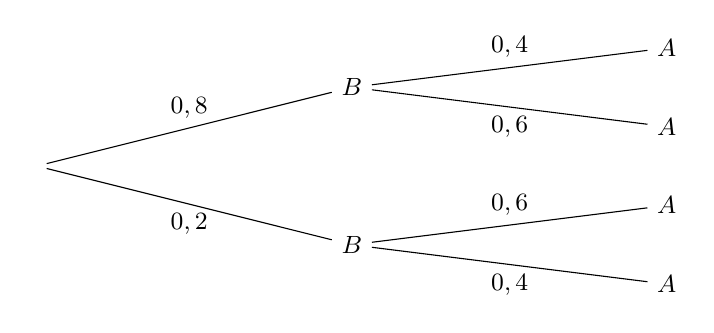
\begin{tikzpicture}[scale=1]
\node {}[grow=right, level distance=4cm, sibling distance=2cm]
	child {node {\small $\widebar{B}$}[level distance=4cm, sibling distance=1cm]
		child {node{\small $\widebar{A}$}
			edge from parent node[below] {\small $0,4$}				
		}
		child {node{\small $A$}
			edge from parent node[above] {\small $0,6$}	
		}
		edge from parent node[below] {\small $0,2$}	
	}
	child {node {\small $B$}[level distance=4cm, sibling distance=1cm]
		child {node{\small $\widebar{A}$}
			edge from parent node[below] {\small $0,6$}	
		}
		child {node{\small $A$}
			edge from parent node[above] {\small $0,4$}
		}
		edge from parent node[above] {\small $0,8$}	
	}
;
\end{tikzpicture}
\end{center}
\begin{multicols}{2}
\item $P(A \cap B) = 0,8 \times 0,4 = 0,32$.
\item $P(\overline{A} \cap \overline{B}) = 0,4 \times 0,2 = 0,08$.
\item $P(A) = 0,8 \times 0,4 + 0,2 \times 0,6 = 0,44$.
\item $P_A(B) = \dfrac{P(B)}{P(A)} P_B(A) = \dfrac{0,8}{0,44} \times 0,4 \approx 0,73$.
\end{multicols}
\end{enumerate}
}

\exe{5}{
Des scientifiques s'intéressent à la population de poissons d'un lac.
Sur les 2~250 individus, 480 sont des ombles, le reste sont des poissons chats.
Parmi les poissons chats, 910 sont des femelles. Il y a en tout 1~300 poissons femelles.
\begin{enumerate}
\item Compléter le tableau croisé d'effectifs ci-dessous :
	\begin{center}
	%\def\arraystretch{1.8}
	\setlength\tabcolsep{20pt}
	\tableaucroise{Femelle & Male & Total}{Omble & & &}{Poisson chat & & &}{Total &&&}
	\end{center}
\item Un scientifique pêche aléatoirement un poisson du lac, estimer (à $10^{-2}$ près) :
\begin{enumerate}
\item la probabilité de pêcher un poisson chat ;
\item la probabilité de pêcher un omble sachant que le poisson est un mâle ;
\item la probabilité de pêcher un poisson chat sachant que le poisson est un mâle.
\end{enumerate}
\item Les évènements \og pêcher un mâle \fg{} et \og pêcher un poisson chat \fg{} sont-ils indépendants ? Justifier.
\end{enumerate}
}{exe:2b}{
\begin{enumerate}
\item
	\begin{center}
	%\def\arraystretch{1.8}
	\setlength\tabcolsep{20pt}
	\tableaucroise{Femelle & Male & Total}{Omble & 390 & 90 & 480}{Poisson chat & 910 & 860 & 1~770}{Total & 1~300 & 950 & 2~250}
	\end{center}
\item
\begin{enumerate}
\item Environ 79 \%.
\item Environ 9 \%.
\item Environ 91 \%.
\end{enumerate}
\item On voit que la probabilité de pêcher un poisson chat et la probabilité de pêcher un poisson chat sachant que c'est un mâle
sont différentes, donc non les évènements sont dépendants.
\end{enumerate}
}

\exe{5}{
On observe un chat. On constate que si la journée est ensoleillée, il chasse (et capture) un lézard 8 fois sur 10. 
Sinon, il n'attrape un lézard que 4 fois sur 10.
On note $p$ la probabilité que la journée soit ensoleillée ainsi que $E$ et $L$ les évènements :
\begin{enumerate}[label=(\roman*)]
\item E : \og la journée est ensoleillée \fg{};
\item L : \og le chat attrape un lézard \fg.
\end{enumerate}
\begin{enumerate} 
\item Construire l'arbre pondéré représentant cette situation.
\item Montrer que $P(L) = 0,4p + 0,4$.
\item On consate que dans 60 \% des cas, le chat attrape un lézard.
\begin{enumerate}
\item Calculer la valeur de $p$. 
\item Sachant qu'il y a 365 jours dans l'année, estimer le nombre de jours ensoleillés. 
\end{enumerate}
\end{enumerate}
}{exe:3b}{
\begin{enumerate} 
\item 

\begin{center}
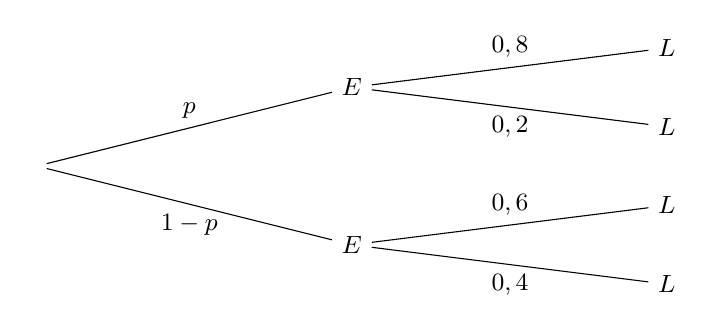
\begin{tikzpicture}[scale=1]
\node {}[grow=right, level distance=4cm, sibling distance=2cm]
	child {node {\small $\widebar{E}$}[level distance=4cm, sibling distance=1cm]
		child {node{\small $\widebar{L}$}
			edge from parent node[below] {\small $0,4$}			
		}
		child {node{\small $L$}
			edge from parent node[above] {\small $0,6$}	
		}
		edge from parent node[below] {\small $1-p$}
	}
	child {node {\small $E$}[level distance=4cm, sibling distance=1cm]
		child {node{\small $\widebar{L}$}
			edge from parent node[below] {\small $0,2$}
		}
		child {node{\small $L$}
			edge from parent node[above] {\small $0,8$}
		}
		edge from parent node[above] {\small $p$}
	}
;
\end{tikzpicture}
\end{center}

\item On a 
\[ P(L) = P(L \cap E) + P(L \cap \overline{E}) = 0,8p + 0,4(1-p) = 0,4p + 0,4 . \]
\item 
\begin{enumerate}
\item Si $P(L) = 0,6$ alors $0,6 = 0,4p + 0,4$ et $p=0,5$.
\item Environ la moitié de l'année soit 183 jours.
\end{enumerate}
\end{enumerate}
}

\exe{5}{
Des sportifs passent un contrôle anti-dopage à l'issue d'une compétition sportive. On considère les deux évènements suivants :
\begin{enumerate}[label=(\roman*)]
\item
$D$ : \og Le sportif est dopé \fg. 
\item
$T$ : \og Le résultat du test est positif \fg. 
\end{enumerate}
La probabilité qu'un sportif soit testé positif sachant qu'il est dopé est de 95 \%. \\
La probabilité qu'un sportif soit testé positif sachant qu'il n'est pas dopé est de 5\%.
\begin{enumerate}
\item On donne $P(D \cap T) = 0,038$ en déduire $P(D)$.
\item Représenter la situation par un arbre de probabilité.
\item Calculer la probabilité qu'un sportif soit testé positif.
\item Calculer la probabilité d'un sportif soit dopé sachant qu'il est testé positif.
\item Commenter la qualité du test mis en oeuvre.
\end{enumerate}
}{exe:4b}{
\begin{enumerate}
\item On a :
\[ P(D \cap T) = P_D(T) \cdot P(D) =  0,019 \] 
avec $P_D(T) = 0,95$, soit : 
\[ P(D) = \dfrac{0,038}{0,95} = 0,04 . \] 
\item 
\begin{center}
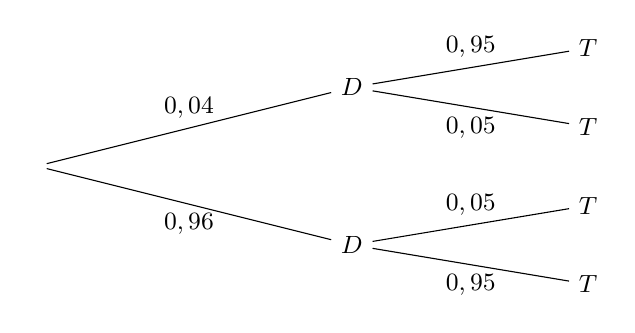
\begin{tikzpicture}[
  grow=right,
  level 1/.style={level distance=4cm, sibling distance=2cm},
  level 2/.style={level distance=3cm, sibling distance=1cm},
]

\node {}
	child {
		node {\small $\widebar{D}$}
		child {
			node {\small $\widebar{T}$}
			edge from parent node[below] {\small $0,95$}
		}
		child {
			node {\small $T$}
			edge from parent node[above] {\small $0,05$}
		}
		edge from parent node[below] {\small $0,96$}
	}
	child {
		node {\small $D$}
		child {
			node {\small $\widebar{T}$}
			edge from parent node[below] {\small $0,05$}
		}
		child {
			node {\small $T$}
			edge from parent node[above] {\small $0,95$}
		}
		edge from parent node[above] {\small $0,04$}
	};
\end{tikzpicture}
\end{center}
\item On a $P(T) = 0,04 \times 0,95 + 0,96 \times 0,05 = 0,086$
\item On cherche $P_T(D)$, on utilise la formule de Bayes :
\[ P_T(D) = \dfrac{P(D)}{P(T)} P_D(T) = \dfrac{0,04}{0,086} \times 0,95 \approx 0,44 . \]
\item Si le test est positif, la probabilité que le sportif soit dopé est seulement de 44 \%, le test est plutôt imprécis.
\end{enumerate}
}

%%%%%%%%%%%%%

\newpage
\fancyhead[C]{\textbf{Solutions}}
Les solutions sont données dans l'ordre sujet a puis b. \newline
\shipoutAnswer


\end{document}
